\documentclass[10pt,twocolumn]{article}
\usepackage{geometry}
\geometry{verbose,headsep=3cm,tmargin=2.5cm,bmargin=2.5cm,lmargin=2.0cm,rmargin=2.0cm}
\usepackage{graphicx}
\usepackage{xcolor}
\usepackage[font=small]{caption}
\usepackage{amsmath,amssymb,latexsym}
\usepackage{marvosym}
\usepackage{url}
\usepackage{lipsum}
\usepackage{bm}
\usepackage{float}
\usepackage[english]{babel}
\usepackage{hyperref}
\usepackage{epsf}
\usepackage{float}
\usepackage{mathpazo}
\usepackage{pifont}
\usepackage{wrapfig}
\usepackage{multicol}
\usepackage{enumitem}
\usepackage{xcolor}
\usepackage{framed}
\usepackage[utf8]{inputenc}
\graphicspath{{DWGs/}}

% Document font:
\usepackage{charter}

\newcommand{\highlight}[1]{%
  \colorbox{orange!50}{$\displaystyle#1$}}
\definecolor{lgray}{cmyk}{0.2,0.2,0.2,0}
\definecolor{llgray}{cmyk}{0.1,0.1,0.1,0}
\definecolor{dgray}{cmyk}{0.3,0.3,0.3, 0}

\begin{document}

%%% HEADER --------------------------------------------------------------
% ------------------------------------------------------------------------

\twocolumn[{
\begin{@twocolumnfalse}

  \begin{center}
%\textcolor{lgray}
    \vskip-5em

    \hfill
    \fontsize{10}{10}\selectfont {\textit{Bruxelles, February 2019}}

    \vskip2ex
    
	\vspace{5ex}
	
    \fontsize{24}{10}\selectfont {Condensed Notes on Combustion}

  \noindent%
    
\vskip1ex

{\rule{\textwidth}{0.5pt}}

  \end{center}

    \fontsize{7}{10}\selectfont {This work is licensed under the Creative Commons Attribution-NonCommercial-ShareAlike 4.0 International (CC BY-NC-SA 4.0) license.}

\vspace{6mm}

\end{@twocolumnfalse}
}]


%%% HEADER END -----------------------------------------------------------
% ------------------------------------------------------------------------

\vspace{10mm}

\setlength{\parindent}{0cm}

\fontsize{14}{10}\selectfont {Kamila Zdybał}

\vspace{2mm}

\fontsize{8}{10}\selectfont {\textit{Université libre de Bruxelles, kamila.zdybal@ulb.ac.be}}

\fontsize{8}{10}\selectfont {\textit{camillejr.github.io/science-docs, kamila.zdybal@gmail.com}}


\section*{Preface}

These are dense notes on \textit{combustion} concepts. They start from the preliminary notions that are needed in understanding the combustion language. Next, they introduce the elements of \textit{thermodynamics} relevant to the study of combustion, and finally present the governing \textit{differential relations} for \textit{reactive flows} in various systems.

These notes are collected from numerous sources from which I studied combustion theory, the main that are ought to be mentioned are: [\ref{bib:turns}] and [\ref{bib:pitsch}].

If you would like to see computational examples that support concepts presented here, I encourage you to take a look at my other document \textit{Computational examples in transport phenomena with Python}.

\,\,

This document is still in preparation. Please feel free to contact me with any suggestions, corrections or comments.

\tableofcontents

\section{Basic concepts}

\subsection{Species}

A \textit{species} is a general name for any chemical compound that takes role in a chemical reaction. In the context of combustion, the most encountered species are for instance: CO2, CO, H2O, O2, N2, etc.

\subsection{Species mass fraction}

A species mass fraction is a ratio between mass $m_i$ of a particular $i$-th species in the mixture and the total mass of the mixture $m_{TOT}$:

\begin{equation}
Y_i = \frac{m_i}{m_{TOT}}
\end{equation}

\subsection{Species mole fraction}

A species molar fraction is the ratio between number of moles $N_i$ of a particular $i$-th species in the mixture and the total number of moles of the mixture $N_{TOT}$:

\begin{equation}
\chi_i = \frac{N_i}{N_{TOT}}
\end{equation}

\subsection{Mass-basis and molar-basis}

In combustion, we encounter both \textit{mass-basis} and \textit{molar-basis} quantities. According to [\ref{bib:pitsch}], the mass-basis is useful because mass is conserved and molar-basis is useful because chemical reactions are written per-molar basis.

\subsection{Air-to-fuel ratio}

Air-to-fuel ratio is the ratio between mass of air $m_{air}$ and mass of fuel $m_{fuel}$ in the mixture.

The stoichiometric air-to-fuel ratio:

\begin{equation}
AF_{st} = \Big( \frac{m_{air}}{m_{fuel}} \Big)_{st}
\end{equation}

And a general air-to-fuel ratio for any mixture:

\begin{equation}
AF = \frac{m_{air}}{m_{fuel}}
\end{equation}

\subsection{Equivalence ratio}

The equivalence ratio is the ratio between stoichiometric air-to-fuel ratio and an actual air-to-fuel ratio:

\begin{equation}
\phi = \frac{AF_{st}}{AF}
\end{equation}

When the real mixture has excess air (it is a \textbf{lean} mixture), $\phi < 1$. For \textbf{rich} mixtures $\phi > 1$.

\subsection{Mixture fraction}

In general, when we create an unburnt mixture from fuel and oxidizer streams, the \textit{fuel stream} is composed of fuel and other fuel-impurities and the \textit{oxidizer stream} is composed of oxidizer and other oxidizer-impurities. The mass of the total fuel stream is $m_1$ and the mass of the total oxidizer stream is $m_2$.

The mixture fraction is the ratio between mass of the fuel stream to the total mass of the unburnt mixture:

\begin{equation}
Z = \frac{m_1}{m_{u, TOT}} = \frac{m_1}{m_1 + m_2}
\end{equation}

\begin{figure}[H]
\centering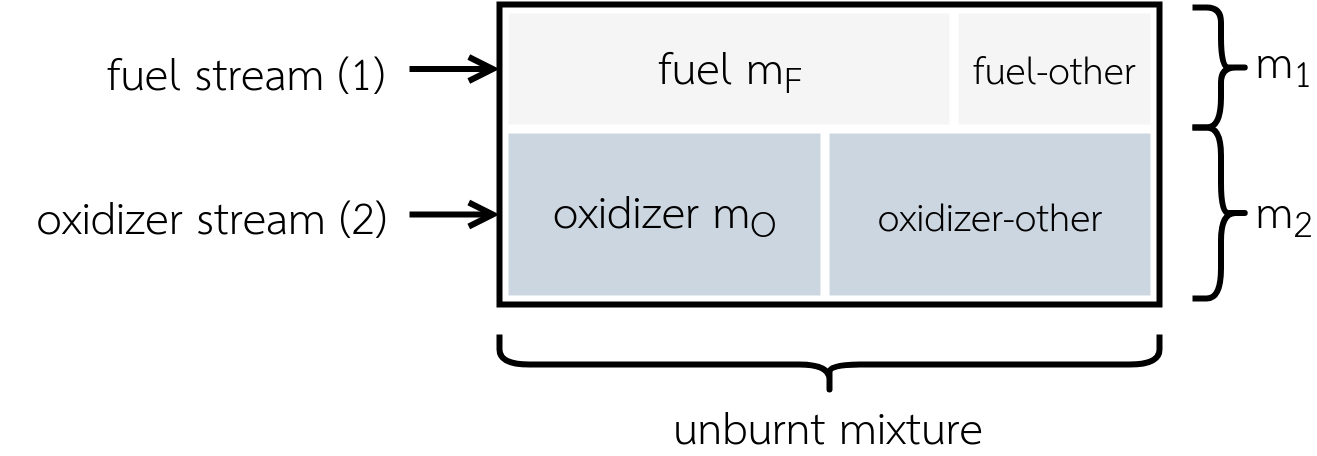
\includegraphics[width=8.5cm]{mixture-fraction.png}
\caption{Fuel-oxidizer stream system.}			
\label{fig:mixture-fraction}
\end{figure}

We may also define the mass fraction of fuel in the unburnt mixture:

\begin{equation}
Y_{u, F} = \frac{m_F}{m_{u, TOT}} = \frac{m_F}{m_1 + m_2}
\end{equation}

and mass fraction of fuel in the fuel stream:

\begin{equation}
Y_{1, F} = \frac{m_F}{m_1}
\end{equation}

These two quantities are clearly related to each other via the mixture fraction:

\begin{equation}
Y_{u, F} = \frac{m_F}{m_1 + m_2} = \frac{m_F}{m_1} \frac{m_1}{m_1 + m_2} = Y_{1, F} Z
\end{equation}

Similar reasoning can be done for the oxidizer in the oxidizer stream.





\subsection{Adiabatic flame temperature}

The adiabatic flame temperature (AdFT) is the temperature of combustion products if the combustion happens without heat exchange with the surroundings. It thus represents the maximum theoretical temperature for a given combustion system.

\subsubsection{Constant pressure AdFT}



\subsubsection{Constant volume AdFT}







\subsection{Dissociation}

The dissociation of a species is the process of spliting that species into smaller particles: either atoms or other species such as ions or radicals.

\section{Energy considerations}

\subsection{Equations of state}

The equation of state owes its name to the fact that it relates variables describing \textit{state} of the system. Among those are: pressure $P$, volume $V$ and temperature $T$.

\begin{equation}
PV = mRT
\end{equation}

\subsubsection{Calorific equation of state}

On the other hand, the calorific equation of state relates internal energy with the state variables.

\begin{equation}
du = \Big( \frac{\partial u}{\partial T} \Big)_V dT + \Big( \frac{\partial u}{\partial V} \Big)_T dV
\end{equation}

\subsection{Thermodynamic potentials}





\subsection{Enthalpy of formation}

The \textit{enthalpy of formation} for a given species is the amount of energy required to form this species from elements in a given state (described by the temperature and pressure).


\subsection{Enthalpy of combustion}

The \textit{enthalpy of combustion} is the amount of heat produced by the combustion process. It is the difference between enthalpy of products and enthalpy of reactants.

\subsection{First law of thermodynamics}

The first law of thermodynamics states, that the total change in energy of the system is equal to the difference of the heat added to the system and work done by the system on the surroundings.



\subsection{Second law of thermodynamics}

The second law of thermodynamics states, that the total entropy of an isolated system can never be negative.

\subsection{Clausius-Clapeyron equation}



\section{Species transport}



\subsection{1-D species transport}

The mechanical transport of species can be twofold: due to a bulk motion of the fluid and/or due to molecular diffusion. Below, we consider one-dimensional binary transport.

\subsubsection{1-D diffusion from Fick's law}

One way to model molecular diffusion is to use Fick's law. It states that the mass flow rate of species $i$ through species $j$ is proportional to the concentration gradient (which is the driving force of diffusion) with the constant $-\rho_i \mathcal{D}_{ij}$:

\begin{equation}
\frac{d \dot{m}_{i, diff}}{dA} = - \rho_i \mathcal{D}_{ij} \frac{d Y_i}{dx}
\end{equation}

The units of the above equation:

\begin{equation*}
\frac{kg}{s \cdot m^2} = \frac{kg}{m^3} \frac{m^2}{s} \frac{1}{m}
\end{equation*}

In the 1-D case, the quantity $\mathcal{D}$ is called \textit{binary diffusivity} and its units are $m^2/s$. In the above equation, $\dot{m}_{i, diff}$ is the mass flux of species due to diffusion, $\rho_i$ is the density of species $i$ and $Y_i$ is the concentration of species.

\subsubsection{1-D bulk flow}

The bulk transport of species $i$ is simply the fraction of the total mixture mass flux that contributes to the transport of that species $i$. That fraction is equal to the mass fraction $Y_i$ of species $i$.

\begin{equation}
\frac{d \dot{m}_{i, bulk}}{dA} = Y_i \frac{d \dot{m}_{TOT}}{d A}
\end{equation}

\subsubsection{1-D binary transport}

For a one-dimensional, binary diffusion (diffusion between two species A and B) we have the mass flow rate of species A per unit area described as:

\begin{equation}
\frac{d \dot{m}_A }{dA} = \frac{d \dot{m}_{A, bulk}}{dA} + \frac{d \dot{m}_{A, diff}}{dA} = Y_A \frac{d \dot{m}_{TOT}}{d A} - \rho_A \mathcal{D}_{AB} \frac{dY_A}{dx}
\end{equation}\label{eq:1d-bin-diff}

where $\dot{m}_{TOT} = \dot{m}_A + \dot{m}_B$.

It is worth mentioning here, that the above result does not yet contain information about possible chemical reactions in which species A and B might take part. The eq.(\ref{eq:1d-bin-diff}) describes only the pure transport of species.

\subsubsection{1-D species conservation}

Differential relations for one-dimensional species conservation can be derived by considering a 1-D control volume $\Delta x$. We now assume that the species can react, and so the mass of a particular species within the control volume can change due to transport, as well as due to creation/destruction of species in a chemical reaction. 

The change of mass of a species A in the control volume can be written as:

\begin{equation}
\frac{d m_{A, CV} }{dt} = \Big[ \frac{d \dot{m}_A}{d A} A \Big]_x - \Big[ \frac{d \dot{m}_A}{d A} A \Big]_{x + \Delta x} + r_A V
\end{equation}

where $r_A$ is the mass production rate of species A per unit volume. For further considerations we will call this term the \textit{source term}.

Substituting $m_{A, CV} = Y_A m_{CV} = Y_A \rho A \Delta x$ we get:

\begin{equation}
A \Delta x \frac{d \rho Y_{A} }{dt} = \Big[ \frac{d \dot{m}_A}{d A} A \Big]_x - \Big[ \frac{d \dot{m}_A}{d A} A \Big]_{x + \Delta x} + r_A A \Delta x
\end{equation}

Using the relation for 1-D binary diffusion from eq.(\ref{eq:1d-bin-diff}), and dividing by $A \Delta x$ we get:

\begin{equation}
\begin{aligned}
\frac{d \rho Y_{A} }{dt} = & \frac{1}{\Delta x}\Big[ Y_A \frac{d \dot{m}_{TOT}}{d A} - \rho \mathcal{D}_{AB} \frac{dY_A}{dx} \Big]_x \\
& - \frac{1}{\Delta x} \Big[ Y_A \frac{d \dot{m}_{TOT}}{d A} - \rho \mathcal{D}_{AB} \frac{dY_A}{dx} \Big]_{x + \Delta x} \\
& + r_A
\end{aligned}
\end{equation}

Finally taking the limit as $\Delta x \rightarrow 0$:

\begin{equation}
\frac{d \rho Y_{A} }{dt} = - \frac{\partial}{\partial x}\Big[ Y_A \frac{d \dot{m}_{TOT}}{d A} - \rho \mathcal{D}_{AB} \frac{dY_A}{dx} \Big] + r_A
\end{equation}






\subsection{Source terms}

\subsection{3-D species transport}

We now extend our previous relations to the 3-D case.

\subsubsection{Reaction rate considerations}

\section{Two views to rule them all}

There are essentially two approaches of describing a reacting system. One is to look at the thermal equilibrium and neglect the description of the stages which led to it. Here, we are only bounded by the laws of thermodynamics. This view does not allow to find its state at any time before the equilibrium has been reached.

Another one, is to involve a chemical mechanism and describe how series of intermediate steps lead to finally reaching a thermal equilibrium. The description will involve much more variables but will also allow, in general, to find a precise state at any given time of the system's evolution towards equilibrium. We will be able to recover the exact path that the chemical species have taken. This is the topic of the next sections.

\section{Chemical kinetics}

\subsection{Reaction rate}






\section{Extension to thermal equations}




\section{Chemical reactors}

A \textit{chemical reactor} is a model for a reacting system. It describes both the geometry, the fluid mechanics/dynamics properties (e.g. when we deal with a reactive flow) and finally it includes a series of physical assumptions about the system.

The quantities that we are interested in finding for a given chemical reactor are temperature function $T(t)$ and the species concentrations $[X_i] = [X_i](t)$. Knowing these two quantities will allow us to make predictions about a given system. It is important to note that the predictions nevertheless cannot exceed the assumptions and limitations of a given reactor. It is in the end an approximation of the reality.

\subsection{Constant pressure, fixed mass reactor}

We look for the solution to two differential equations:

\begin{equation}
\frac{d T(t)}{dt} = f([X_i], T)
\end{equation}

\begin{equation}
\frac{d [X_i](t)}{dt} = f([X_i], T)
\end{equation}

\subsubsection{Temperature}

We start by applying the first law of thermodynamics to the reactor:

\begin{equation}
\frac{du}{dt} = \frac{dq}{dt} - \frac{dw}{dt}
\end{equation}

We then substitute for the values of internal energy (the enthalpy equation) and work (assuming the only work done by the system is in moving the piston):

\begin{equation}
\frac{dh}{dt} = \frac{du}{dt} + P \frac{dv}{dt} \rightarrow \frac{du}{dt} = \frac{dh}{dt} - P \frac{dv}{dt}
\end{equation}

\begin{equation}
w = Pv \rightarrow \frac{d w}{dt} = P \frac{dv}{dt} 
\end{equation}

Substitution gives:

\begin{equation}
\frac{dq}{dt} = \frac{dh}{dt}
\end{equation}

We would like the temperature and species fractions to appear in the equation.

\subsubsection{Species concentrations}








\section{Chemical mechanism reduction}


\subsection{Parametrization of the chemical state space}

\subsubsection{Flamelet model}

The flamelet model parametrizes the $n$-dimensional thermochemical state with two parameters - the mixture fraction $Z$ and the scalar dissipation rate $\chi$. In other words:

\begin{equation}
\text{state} \in {\mathbb{R}^n} = f(Z, \chi)
\end{equation}

The dimensionality is therefore reduced to a pre-described two degrees of freedom.



\thebibliography{}

\bibitem{Turns} S. R. Turns, \textit{An Introduction to Combustion: Concepts and Applications}, Second Edition, 2000 \label{bib:turns}

\bibitem{Pitsch} H. Pitsch, \textit{Combustion Theory and Applications in CFD}, Lecture Series \label{bib:pitsch}

\label{bib:pope}

\end{document}